\subsection{k-Nearest Neighbour (k-NN) Classifier}\index{k-Nearest Neighbour classifier}\index{k-NN}
\label{sec:knn}

Similar to PDE-RS (\cf\  Sec.~\ref{sec:pders}), the k-nearest neighbour method compares 
an observed (test) event to reference events from a training data set~\cite{FriedmanBook}. 
However, unlike PDE-RS, which in its original form uses a fixed-sized multidimensional volume 
surrounding the test event, and in its augmented form resizes the volume as a function of 
the local data density, the k-NN algorithm is intrinsically adaptive. It searches for a 
fixed number of adjacent events, which then define a volume for the metric used. The k-NN 
classifier has best performance when the boundary that separates signal and background 
events has irregular features that cannot be easily approximated by parametric learning 
methods. 

\subsubsection{Booking options}

The k-NN classifier is booked via the command:
\begin{codeexample}
\begin{tmvacode}
factory->BookMethod( Types::kKNN, "kNN", "<options>" );
\end{tmvacode}
\caption[.]{\codeexampleCaptionSize Booking of the k-NN classifier: the first argument is 
		   a predefined enumerator, the second argument is a user-defined 
		   string identifier, and the third argument is the configuration options string.
         Individual options are separated by a ':'. 
         See Sec.~\ref{sec:usingtmva:booking} for more information on the booking.}
\end{codeexample}

The configuration options for the k-NN classifier are listed in Option Table~\ref{opt:mva::knn}
(see also Sec.~\ref{sec:fitting}).

% ======= input option table ==========================================
\begin{option}[t]
\input optiontables/MVA__KNN.tex
\caption[.]{\optionCaptionSize 
     Configuration options reference for MVA method: {\em k-NN}.
     Values given are defaults. If predefined categories exist, the default category 
     is marked by a '$\star$'. The options in Option Table~\ref{opt:mva::methodbase} on 
     page~\pageref{opt:mva::methodbase} can also be configured.     
}
\label{opt:mva::knn}
\end{option}
% =====================================================================

\subsubsection{Description and implementation}

The k-NN algorithm searches for $k$ events that are closest to the test event. Closeness 
is thereby measured using a metric function. The simplest metric choice is the Euclidean 
distance
\beq
   R = \left(\sum_{i = 1}^{\Nvar} |x_{i} - y_{i}|^{2}\right)^{\!\!\frac{1}{2}}\;.
\eeq
where $\Nvar$ is the number of input variables used for the classification, $x_{i}$ are 
coordinates of an event from a training sample and $y_{i}$ are variables of an observed 
test event. The $k$ events with the smallest values of $R$ are the {\em k-nearest neighbours}. 
The value of $k$ determines the size of the neighbourhood for which a probability density 
function is evaluated. Large values of $k$ do not capture the local behavior of the 
probability density function. On the other hand, small values of $k$ cause statistical
fluctuations in the probability density estimate. A case study with real data suggests 
that values of $k$ between 10 and 100 are appropriate and result in similar classification 
performance when the training sample contains hundreds of thousands of events (and $\Nvar$
is of the order of a few variables).

The classification algorithm finds k-nearest training events around a query point
\beq
   k = k_{S} + k_{B}\;,
\eeq
where $k_{S(B)}$ is number of the signal (background) events in the training sample. 
The relative probability that the test event is of signal type is given by
\beq
   P_{S} = \frac{k_{S}}{k_{S} + k_{B}} = \frac{k_{S}}{k}\;.
\eeq
The choice of the metric governs the performance of the nearest neighbour algorithm. 
When input variables have different units a variable that has a wider distribution 
contributes with a greater weight to the Euclidean metric. This feature is compensated 
by rescaling the variables using a scaling fraction determined by the option \code{ScaleFrac}.
Rescaling can be turned off by setting \code{ScaleFrac} to 0. The scaling factor applied
to variable $i$ is determined by the width $w_{i}$ of the $x_{i}$ distribution for the 
combined sample of signal and background events: $w_{i}$ is the interval that contains 
the fraction \code{ScaleFrac} of $x_{i}$ training values. The input variables are 
then rescaled by $1/w_{i}$, leading to the rescaled metric
\beq
   R_{\rm rescaled} = 
   \left(\sum_{i = 1}^{d} \frac{1}{w_{i}^{2}}|x_{i} - y_{i}|^{2}\right)^{\!\!\frac{1}{2}}\;. 
\eeq
\begin{figure}[t]
  \begin{center}
    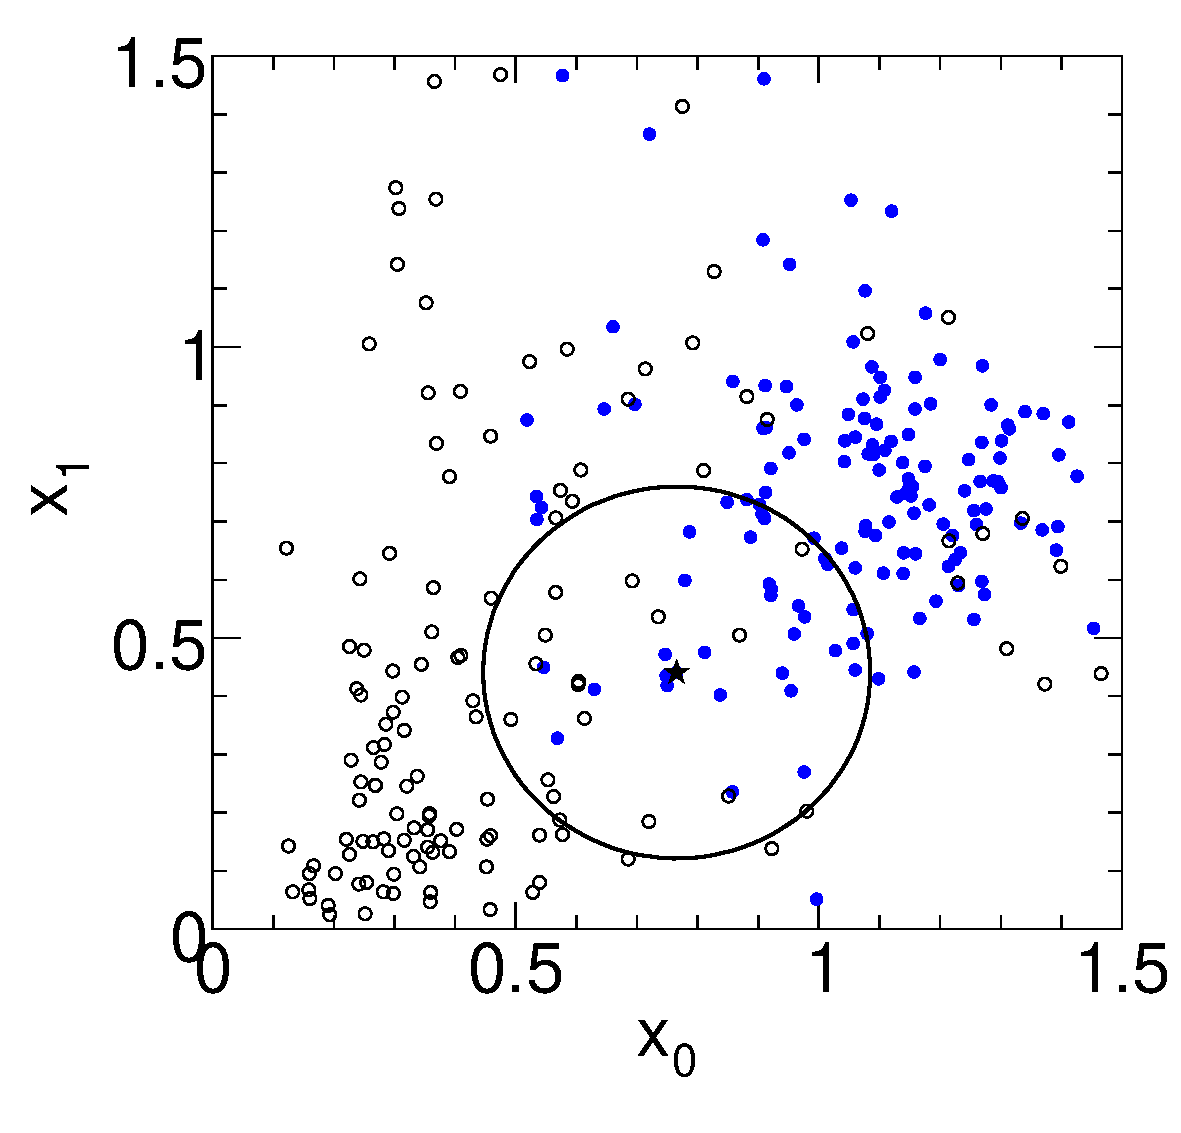
\includegraphics[width=0.325\textwidth]{plots/knn_3d_s13_b7_x01}
    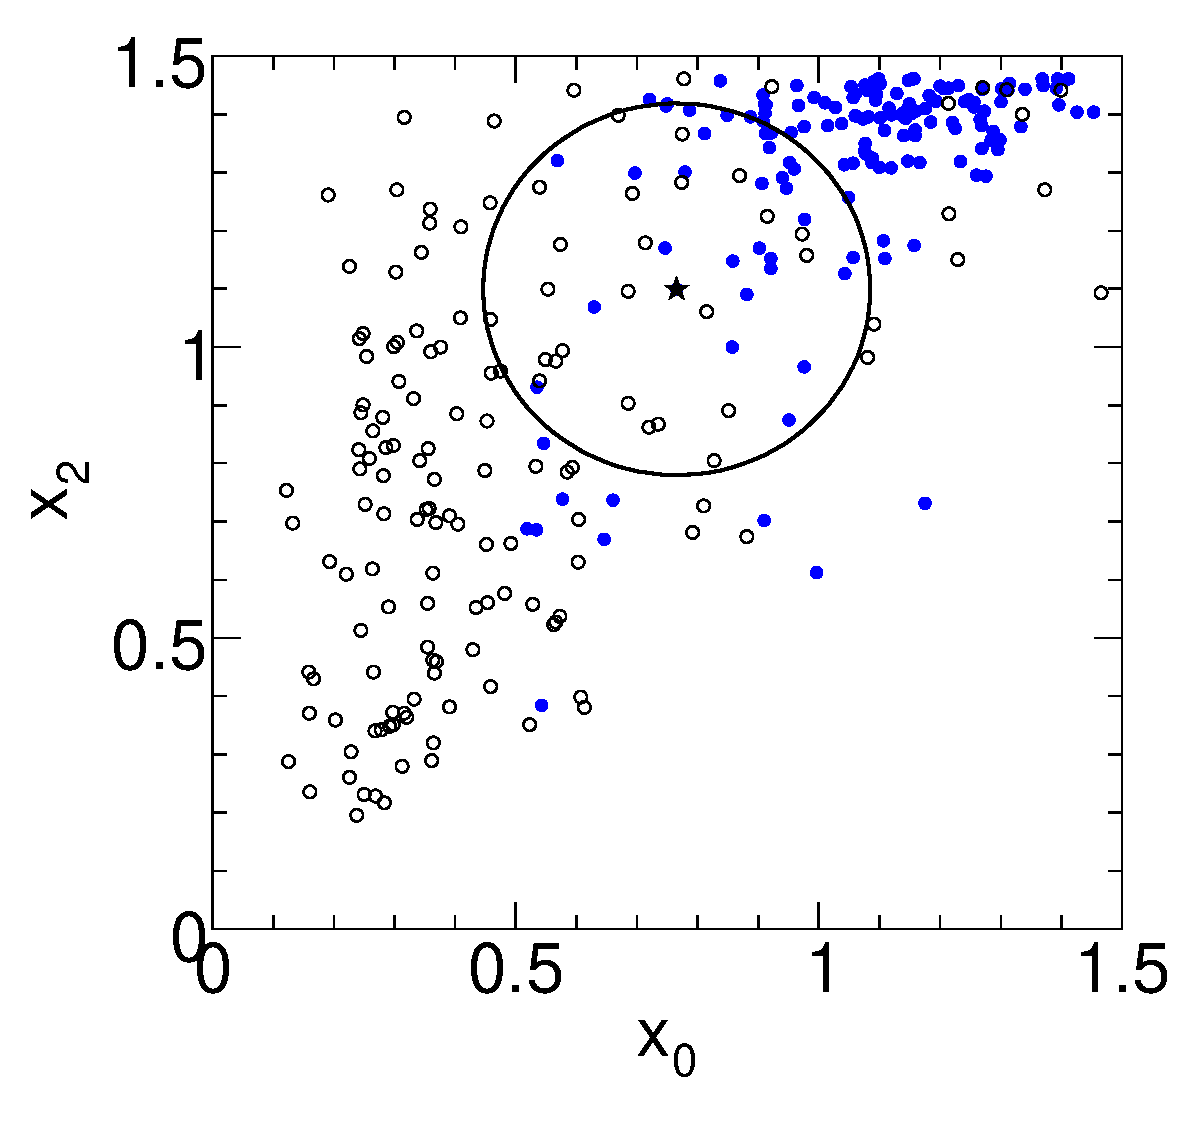
\includegraphics[width=0.325\textwidth]{plots/knn_3d_s13_b7_x02}
    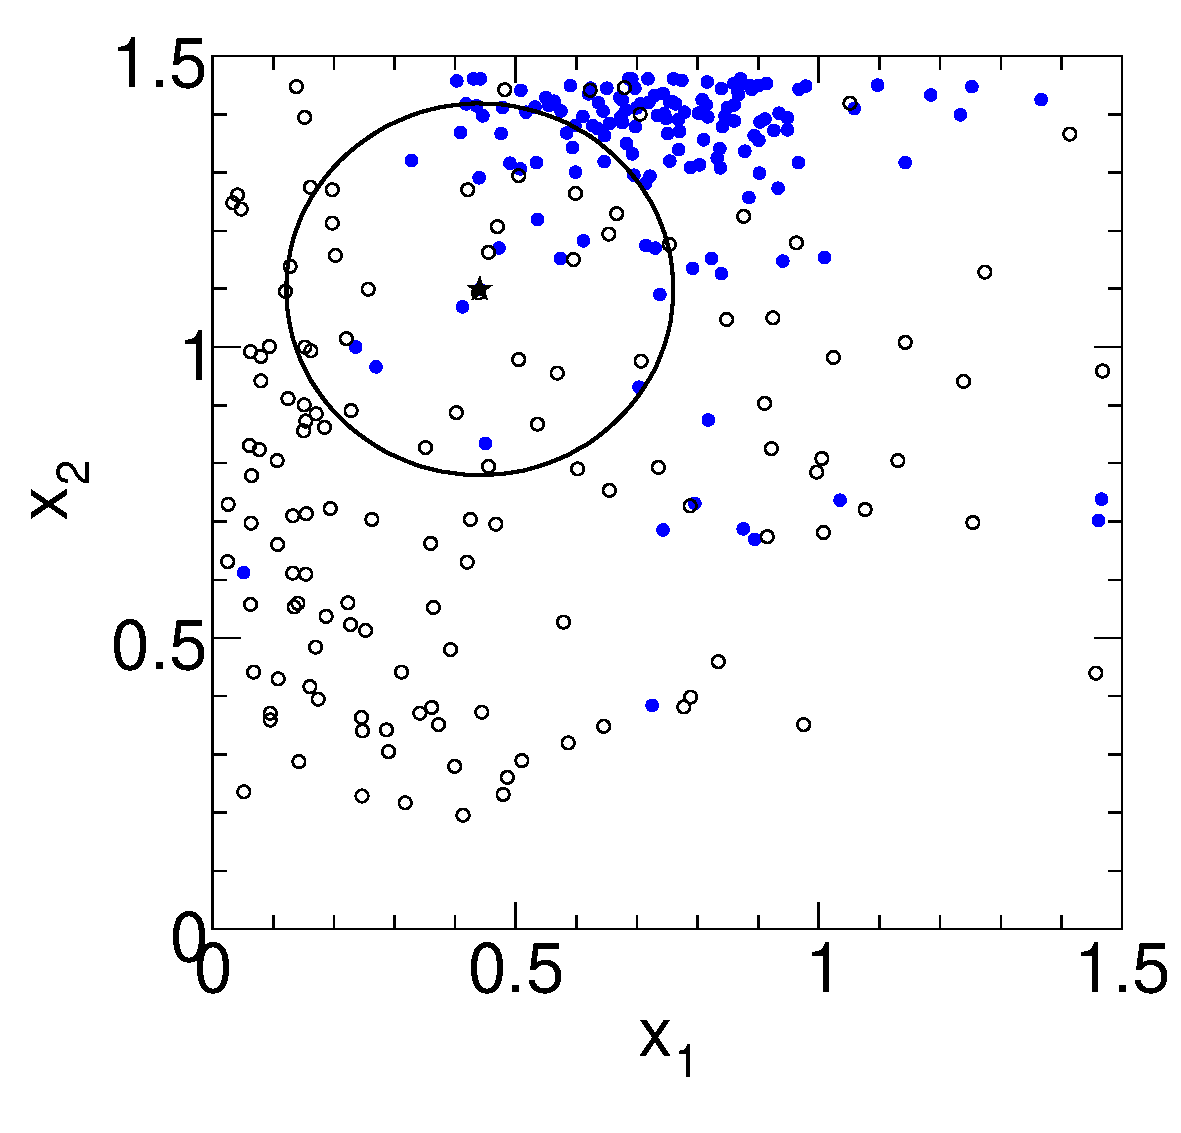
\includegraphics[width=0.325\textwidth]{plots/knn_3d_s13_b7_x12}
  \end{center}
  \vspace{-0.7cm}
  \caption[.] { Example for the k-nearest neighbour algorithm in a three-dimensional space
                (\ie, for three discriminating input variables). The three plots are 
                projections upon the two-dimensional coordinate planes. The full (open) circles 
                are the signal (background) events. The k-NN algorithm searches for 20 nearest 
                points in the {\em nearest neighborhood} (circle) of the query event, shown as 
                a star. The nearest neighborhood counts 13 signal and 7 background points 
                so that query event may be classified as a signal candidate. }
\label{fig:knn-3d} 
\end{figure}
Figure~\ref{fig:knn-3d} shows an example of event classification with the k-nearest 
neighbour algorithm.\footnote
{
  The number of training events shown has been greatly reduced to illustrate the 
  principle of the algorithm. In a real application a typical k-NN training sample 
  should be ample.
}

The output of the k-nearest neighbour algorithm can be interpreted as a probability 
that an event is of signal type, if the numbers (better: sum of event weights) of 
signal and background events in the training sample are equal. This can be enforced
via the \code{Trim} option. If set training events of the overabundant type are 
randomly removed until parity is achieved.
% Using equal number of signal and background events for the classification allows 
% to measure the relative fractions of signal and background events in the observed 
% data. This way the dependency on the underlying model used to generated training 
% events is removed.

Like (more or less) all TMVA classifiers, the k-nearest neighbour estimate suffers 
from statistical fluctuations in the training data. The typically high variance of the 
k-NN response is mitigated by adding a weight function that depends smoothly on the 
distance from a test event. The current k-NN implementation uses a polynomial kernel
\beq
  W(x) = \left\{\begin{array}{ll}
                  (1 - |x|^{3})^{3} & \text{ if } |x| < 1\;, \\[0.1cm]
                  0 & \text{ otherwise}\;.
                \end{array}     
         \right. 
\eeq
If $R_{k}$ is the distance between the test event and the $k$th neighbour, the events 
are weighted according to the formula:
\beq
  W_{S(B)} = \sum_{i = 1}^{k_{S(B)}} W\left(\frac{R_{i}}{R_{k}}\right)\;,
\eeq
where $k_{S(B)}$ is number of the signal (background) events in the neighbourhood. 
The weighted signal probability for the test event is then given by
\beq
  P_{S} = \frac{W_{S}}{W_{S} + W_{B}}\;.
\eeq
The kernel use is switched on/off by the option \code{UseKernel}.

\subsubsection*{Regression}

The k-NN algorithm in TMVA also implements a simple multi-dimensional (multi-target)
regression model. For a test event, the algorithm finds the k-nearest neighbours 
using the input variables, where each training event contains a regression value. 
The predicted regression value for the test event is the weighted average of the 
regression values of the k-nearest neighbours, \cf Eq.~(\ref{eq:PDERSregratio})
on page~\pageref{eq:PDERSregratio}.

\subsubsection{Ranking}

The present implementation of k-NN does not provide a ranking of the input variables.

\subsubsection{Performance}

The simplest implementation of the k-NN algorithm would store all training events in an array. 
The classification would then be performed by looping over all stored events and finding 
the k-nearest neighbours. As discussed in Sec.~\ref{sec:binaryTrees}, such an implementation
is impractical for large training samples. The k-NN algorithm therefore uses a {\em kd-tree} 
structure~\cite{kd-tree} that significantly improves the performance.

The TMVA implementation of the k-NN method is reasonably fast to allow classification of large 
data sets. In particular, it is faster than the adaptive PDE-RS method (\cf\  Sec.~\ref{sec:pders}).
Note that the k-NN method is not appropriate for problems where the number of input 
variables exceeds $\Nvar\gtrsim 10$. The neighbourood size $R$ depends on $\Nvar$
and the size of the training sample $\Ntrain$ as
\beq
  R_{N} \propto \frac{1}{\sqrt[\Nvar]N}\;.
\eeq
A large training set allows the algorithm to probe small-scale features that distinguish 
signal and background events.

%%% Local Variables: 
%%% mode: latex
%%% TeX-master: "TMVAUsersGuide"
%%% End: 
